\section{Руководство пользователя}
\label{sec:document}

\subsection{Авторизация пользователя в системе}
\label{sec:document:auth}

Предоставление определённому лицу или группе лиц прав на выполнение определённых действий, а также процесс подтверждения данных прав при попытке выполнения этих действий, начинается с шага, изображенного на рисунке~\ref{fig:document:auth:two}, в котором пользователь добавляет или создает новое хранилище.

\begin{figure}[ht]
\centering
  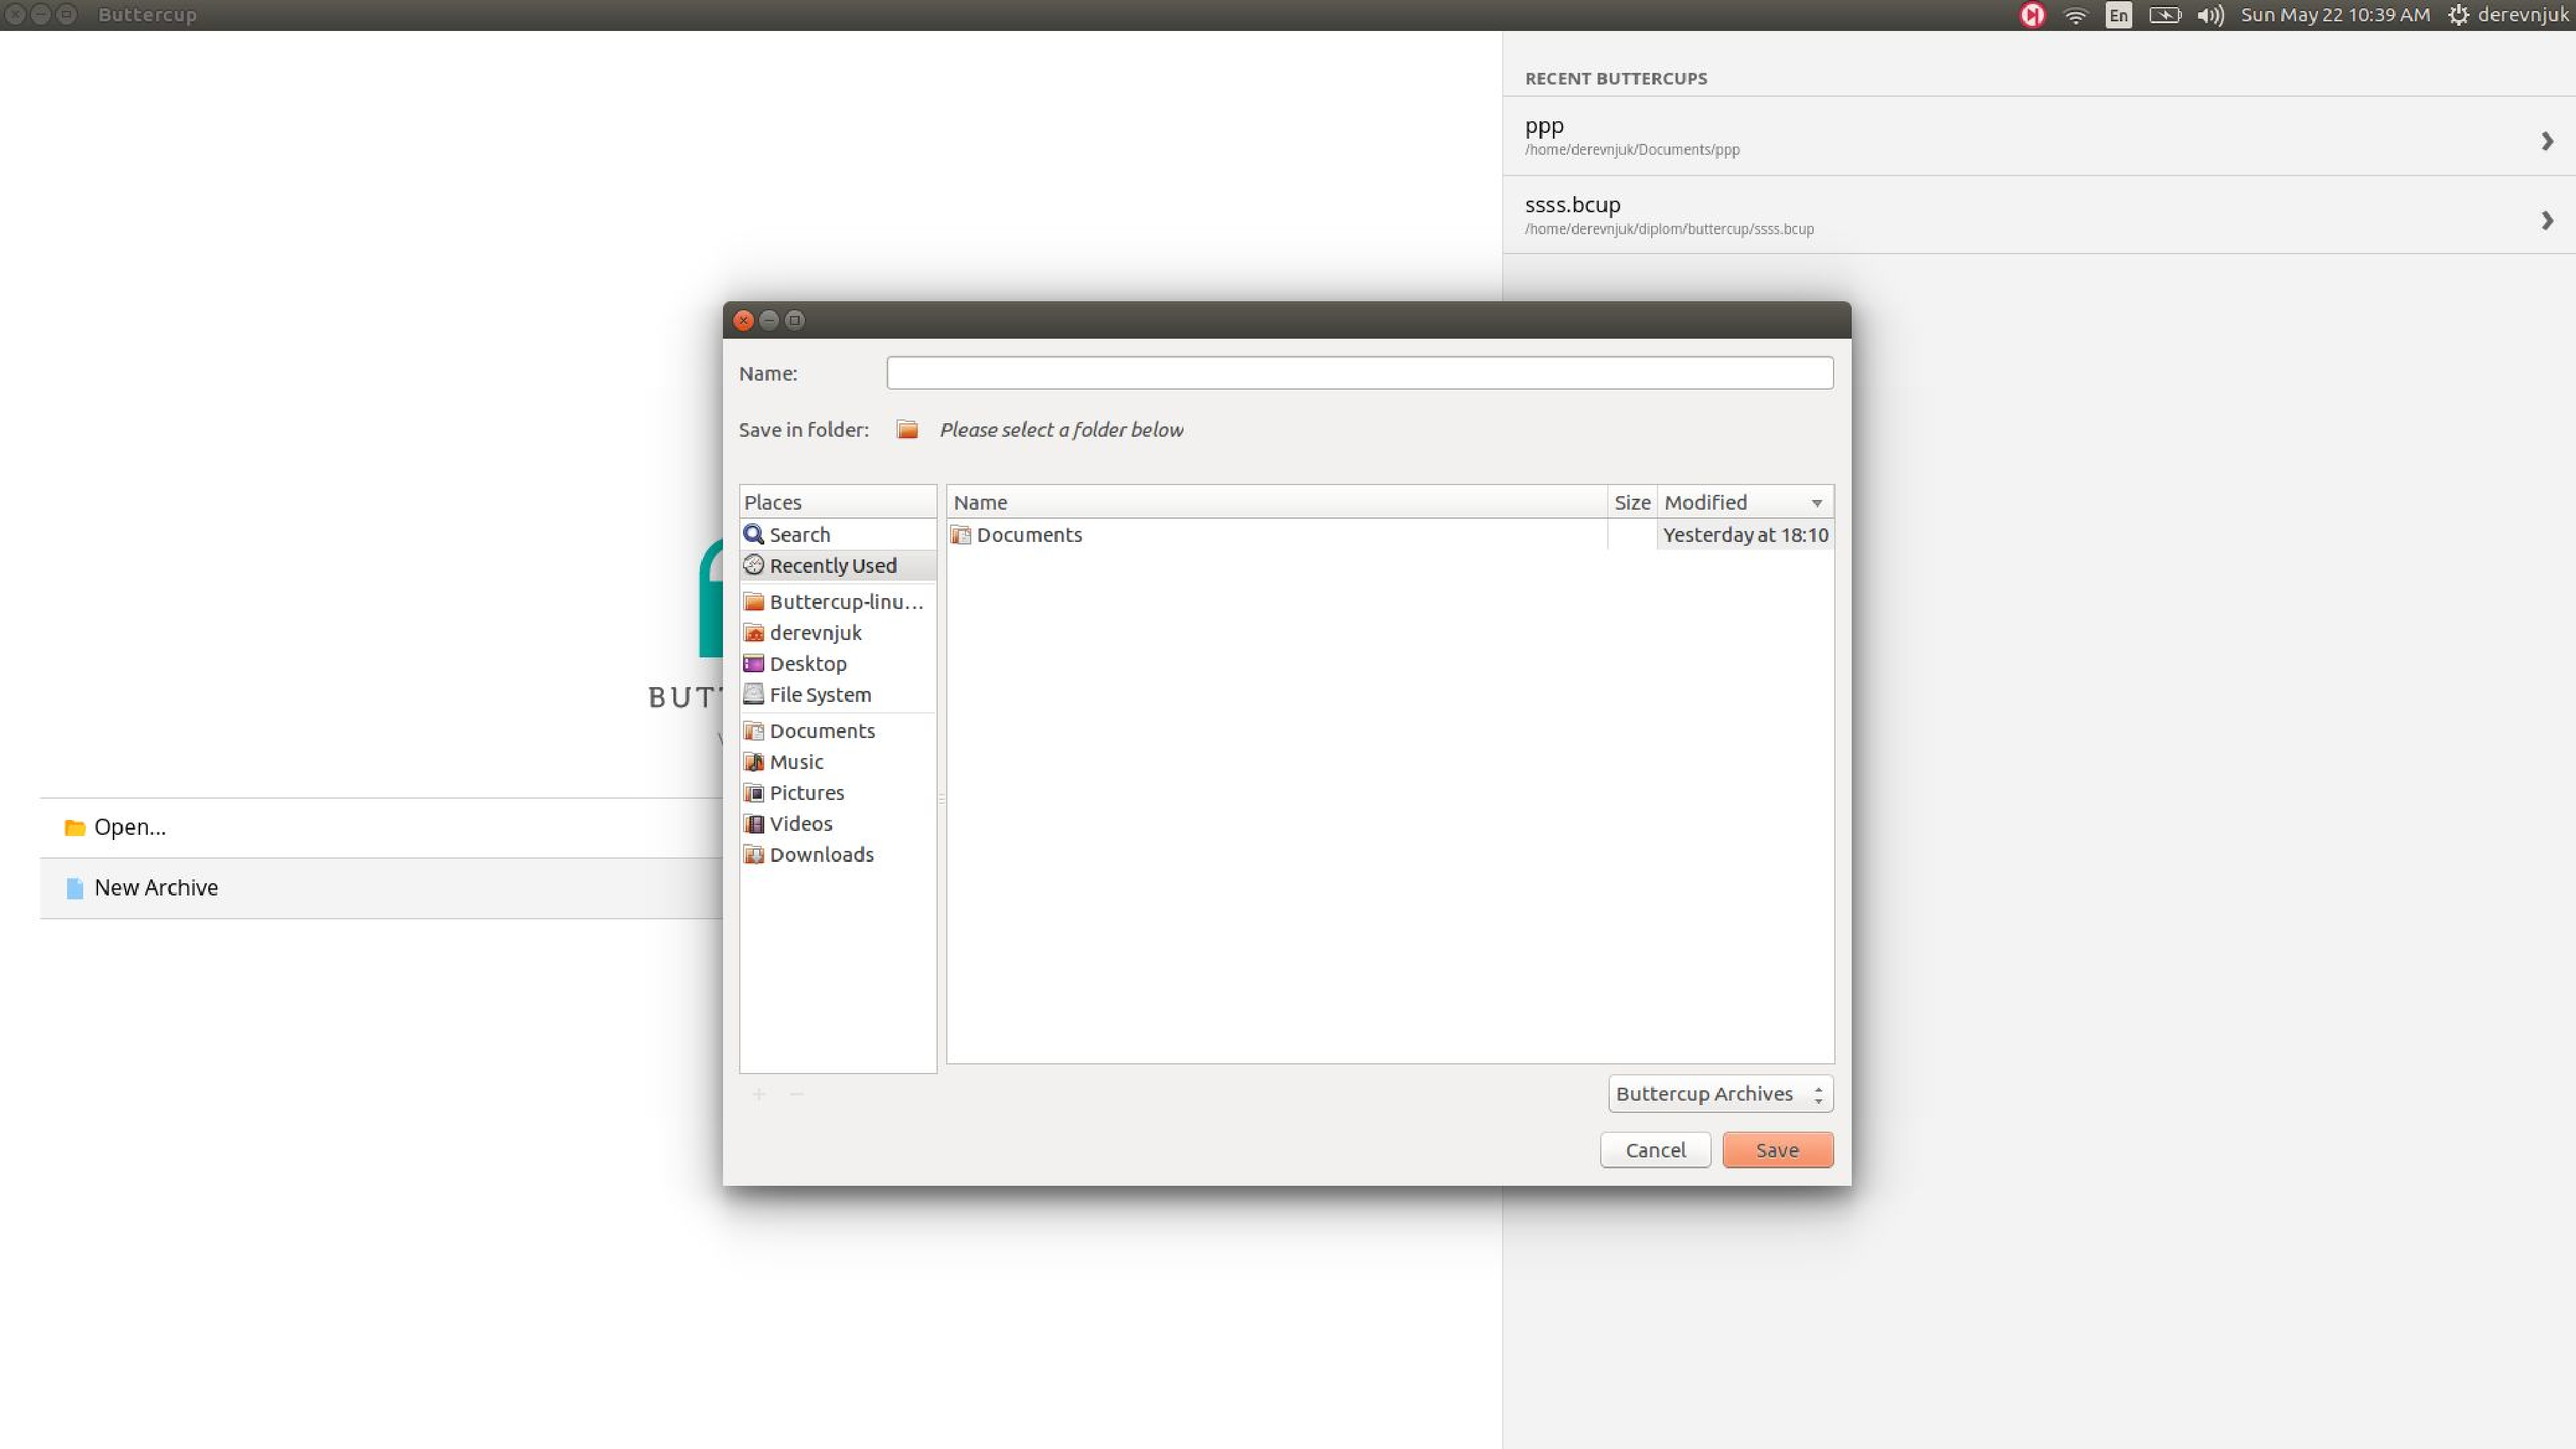
\includegraphics[scale=0.20]{2.pdf}
  \caption{ Окно загрузки/создания хранилища. }
  \label{fig:document:auth:two}
\end{figure}

Пользователь может проверить правильность введенных данных и уйти с формы авторизации через панель активных действий, если передумал. После подтверждения авторизации пользователю предоставляется полный доступ к функционалу системы.

После заполнения полей пользователь переходит ко второму шагу. На нем происходит запрос данных, необходимых для дешифровки и предоставления пользовательских данных. Для входа необходимо ввести один из вариантов логина, пароль доступа и нажать кнопку входа. Также
возможен вход с помощью электронной подписи хранилища. На текущий момент реализован последний подход при аутентификации. Если
пользователь не обладает хранилищем, то следует нажать на кнопку создания хранилища.
После успешного входа откроется главная страница с личными данными пользователя. Представление этого процесса изображено на рисунке~\ref{fig:document:auth:therd}.
\begin{figure}[ht]
\centering
  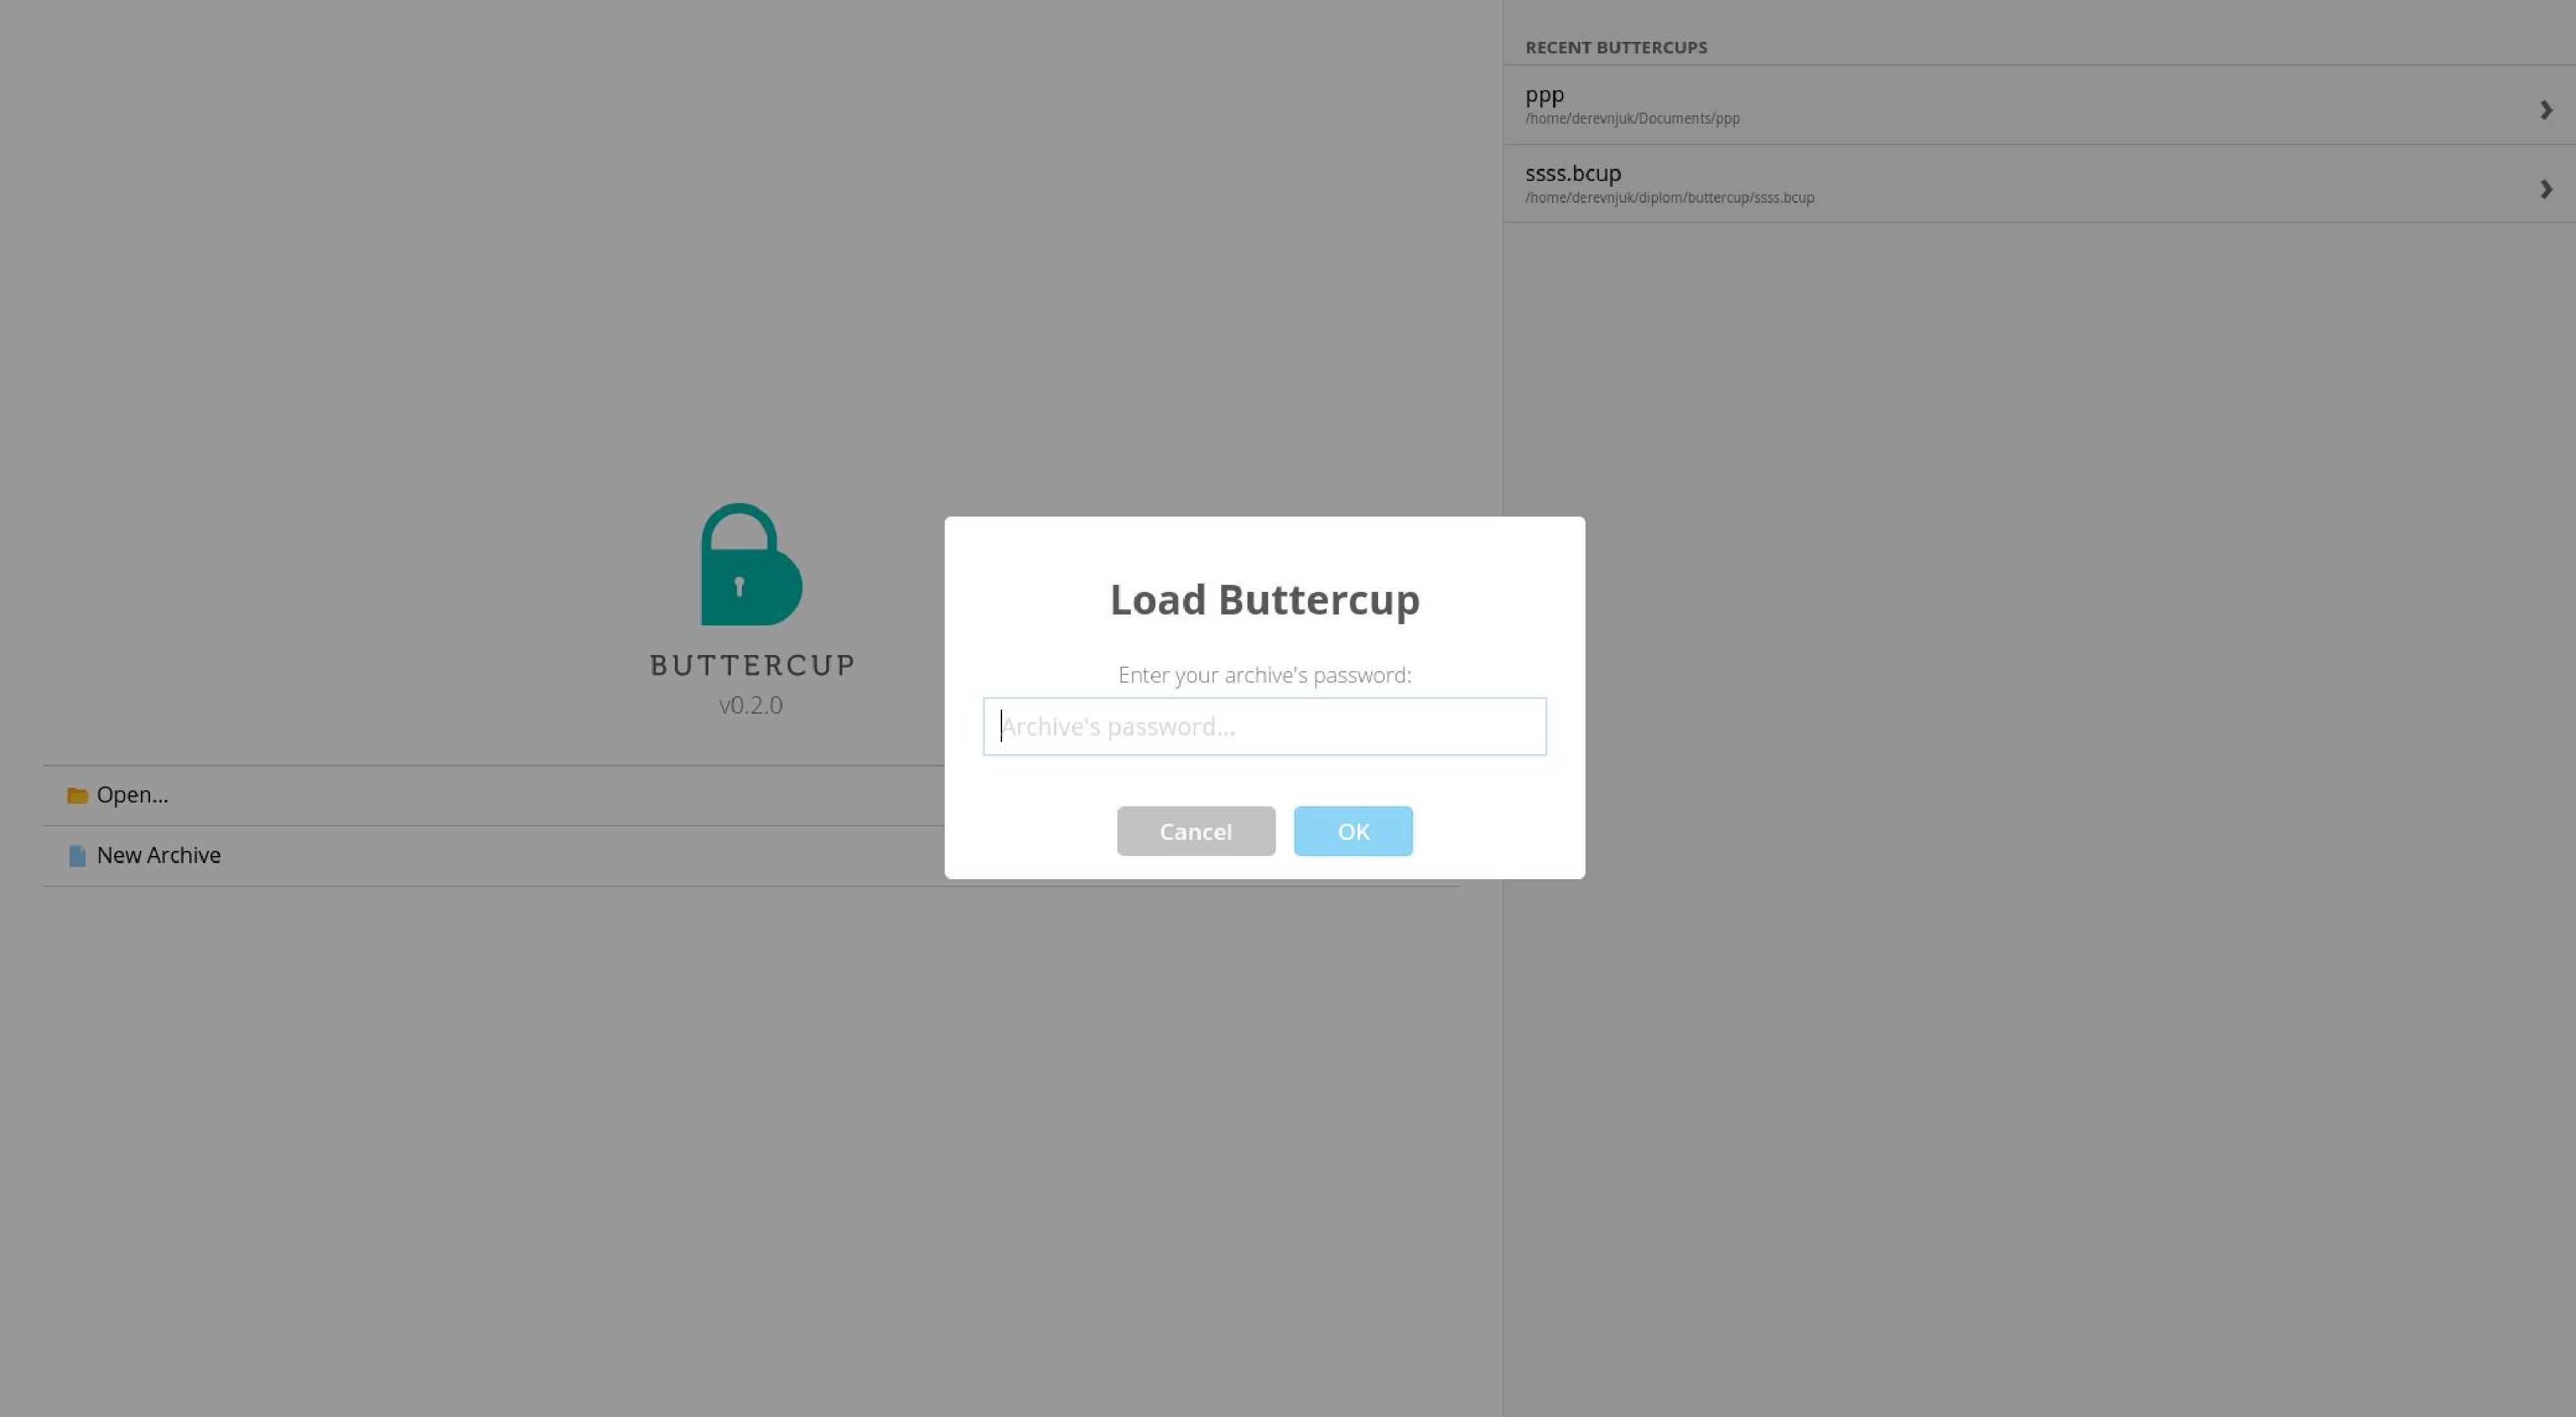
\includegraphics[scale=0.20]{3.pdf}
  \caption{ Окно авторизации пользователя. }
  \label{fig:document:auth:therd}
\end{figure}
\newpage
При загрузке страницы первым делом производится запрос в базу данных с ключами, которые были переданы в метод контроллера. При некорректных ключах, либо при несуществующей записи в базе, пользователь увидит предупреждающий баннер на красном фоне, который изображен на рисунке~\ref{fig:document:auth:nein}.
\begin{figure}[ht]
\centering
  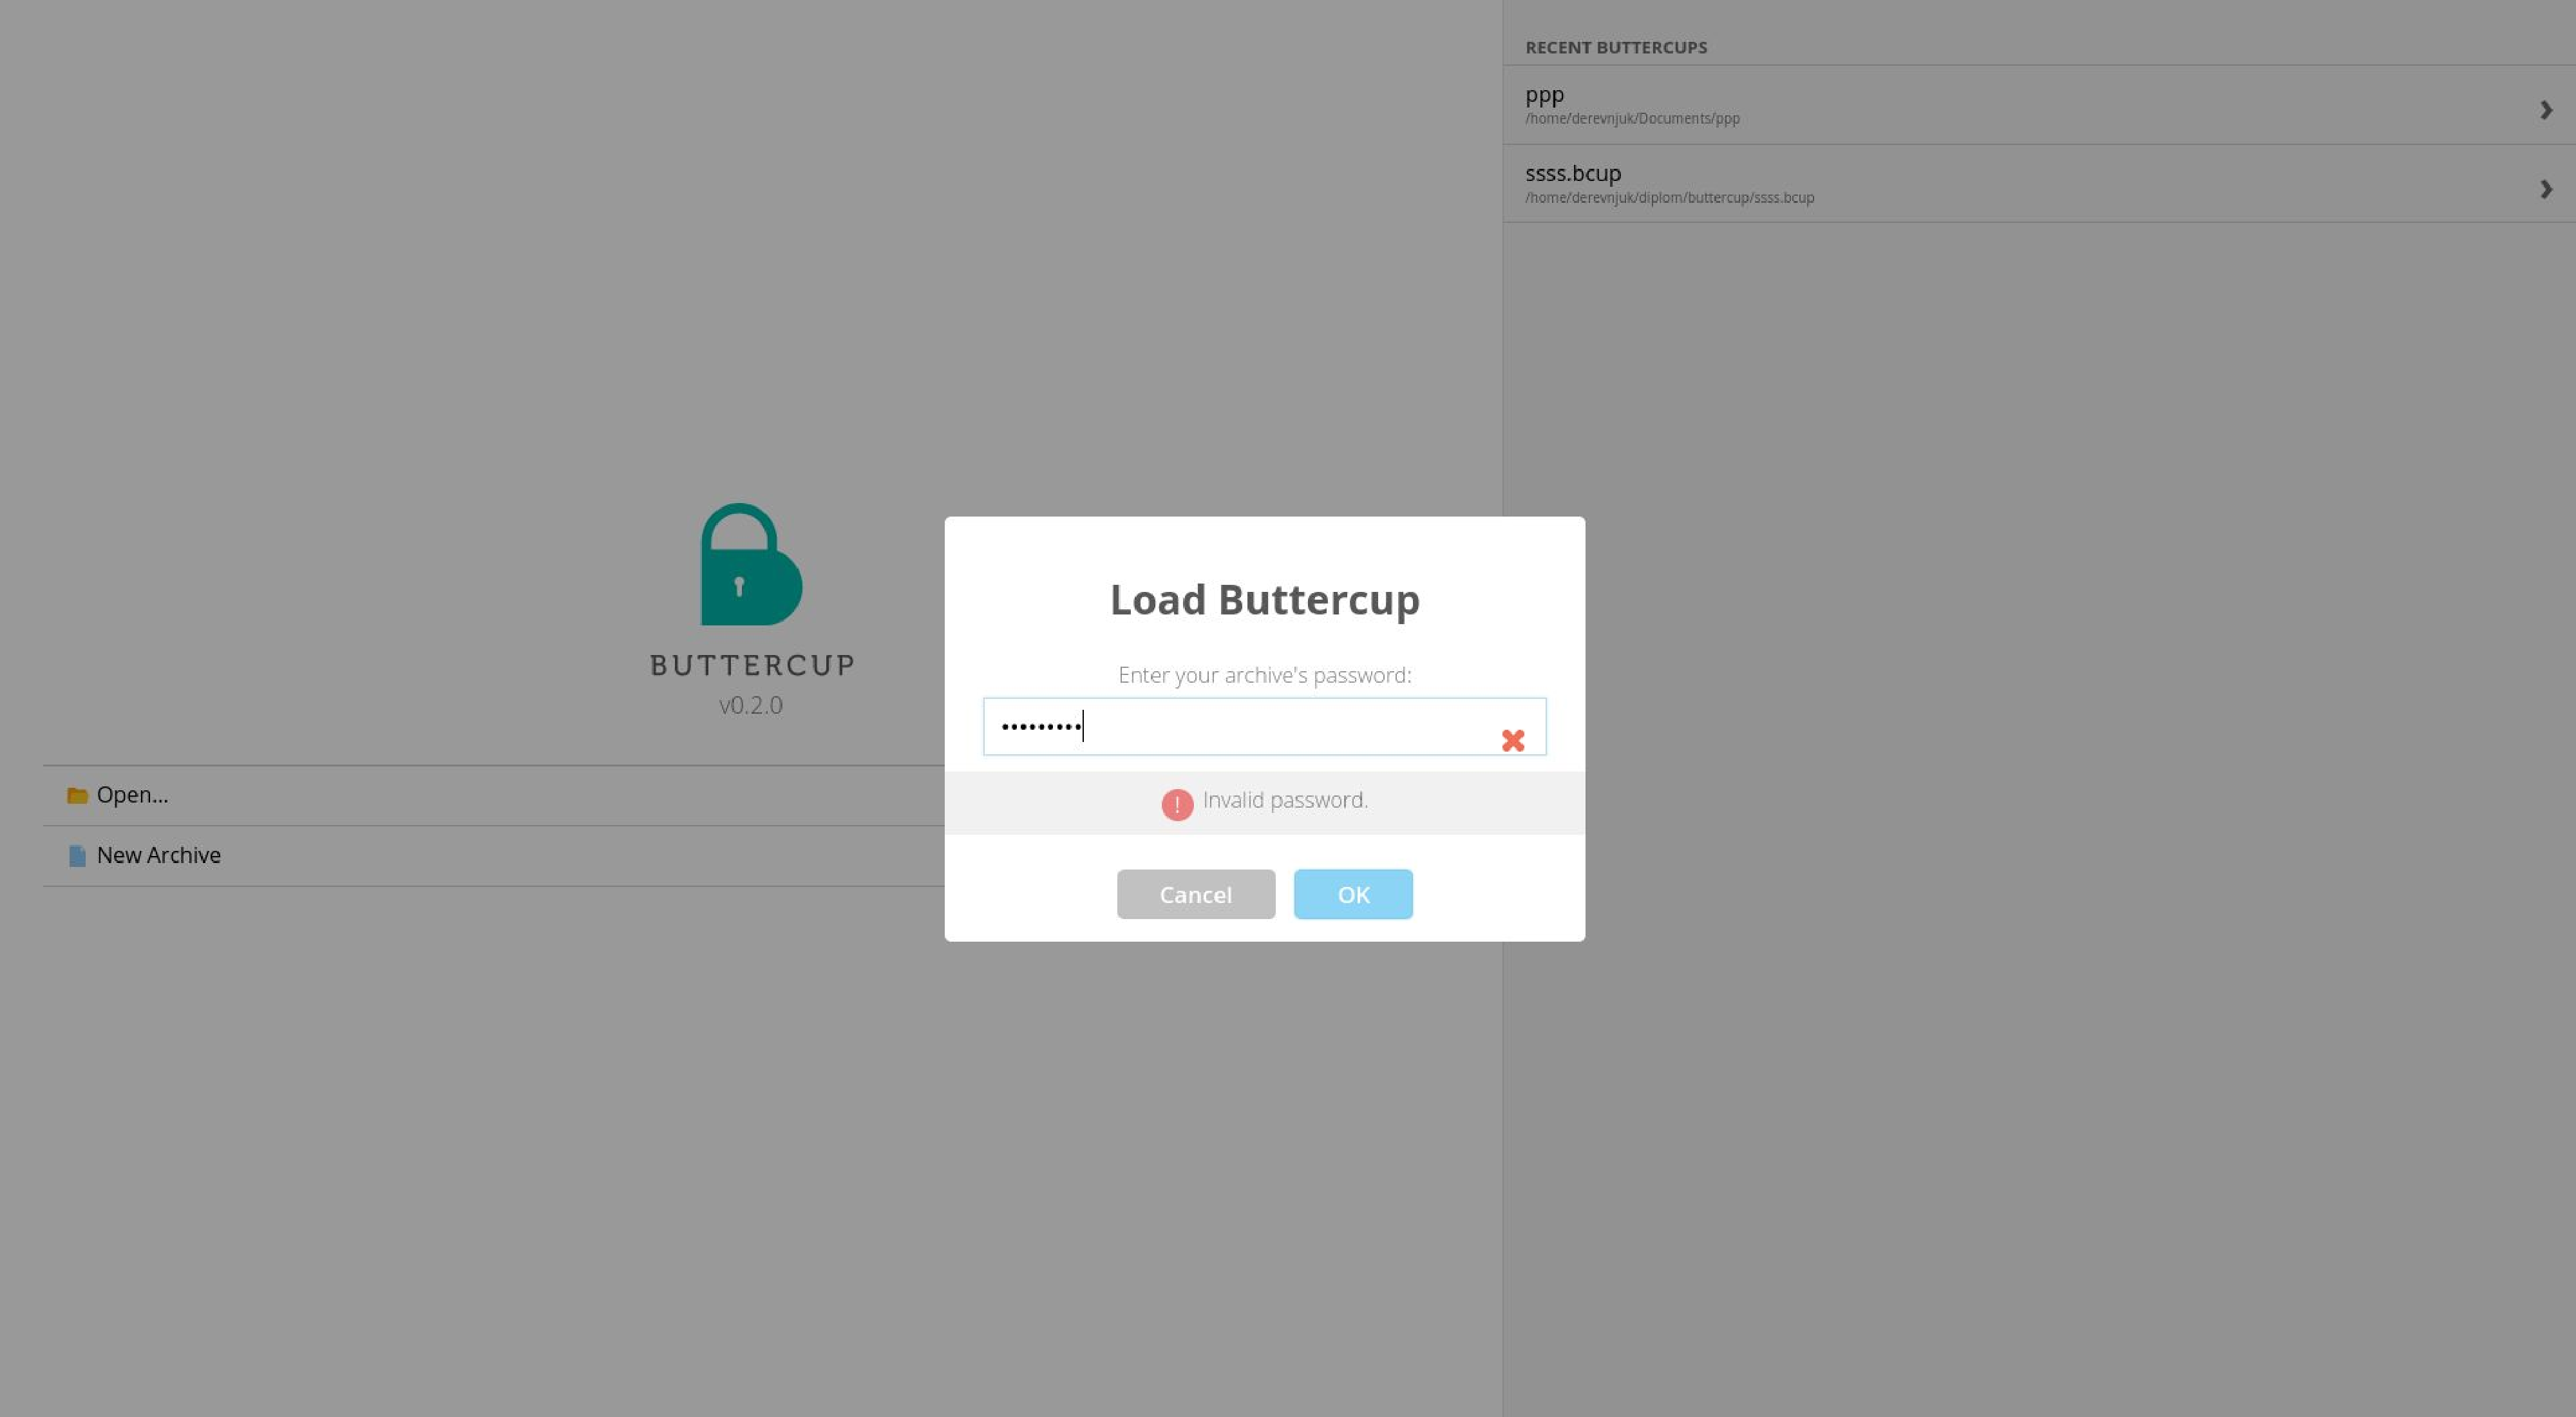
\includegraphics[scale=0.20]{9.pdf}
  \caption{ Окно с неверными ключами. }
  \label{fig:document:auth:nein}
\end{figure}

Предупреждающий баннер на красном фоне, который изображен на рисунке~\ref{fig:document:auth:nein}, является основным элементом обратной связи при вводе некорректных данных в процессе работы с программной.

\subsection{Управление группами в хранилище}
\label{sec:document:created_groupe}

Приложение разработано таким образом, что пользователь не увидит критических сообщений. Все ошибки логируются и сохраняются в базу данных.
Вся работа страницы заключается в управлении и организации составляющих хранилища паролей; в предоставлении доступа к бизнес логике, инкапсулируемой отдельными компонентами.

На основании вышеизложенного, можно выделить шесть основных секций страницы:
\begin{itemize}
	\item дерево группы;
	\item список записей для активной группы;
	\item панель поиска;
	\item область редактора активной записи;
	\item панель активных действий в области групп;
	\item панель активных действий в области записей;
\end{itemize}

Добавление группы в хранилище производится посредством панели активных действий в области групп, которая обращается к собственной валидационной модели. При попытке добавления некорректных данных пользователь получит предупреждение.
Удаление группы в хранилище производится посредством ее собственной панели управления, состоящей из кнопок, предназначенных для удаления и смены ее имени, соотвественно. Процесс удаления группы General, как базовой группы хранилища, представлен на рисунке~\ref{fig:document:created_group:eith}.
\begin{figure}[ht]
\centering
  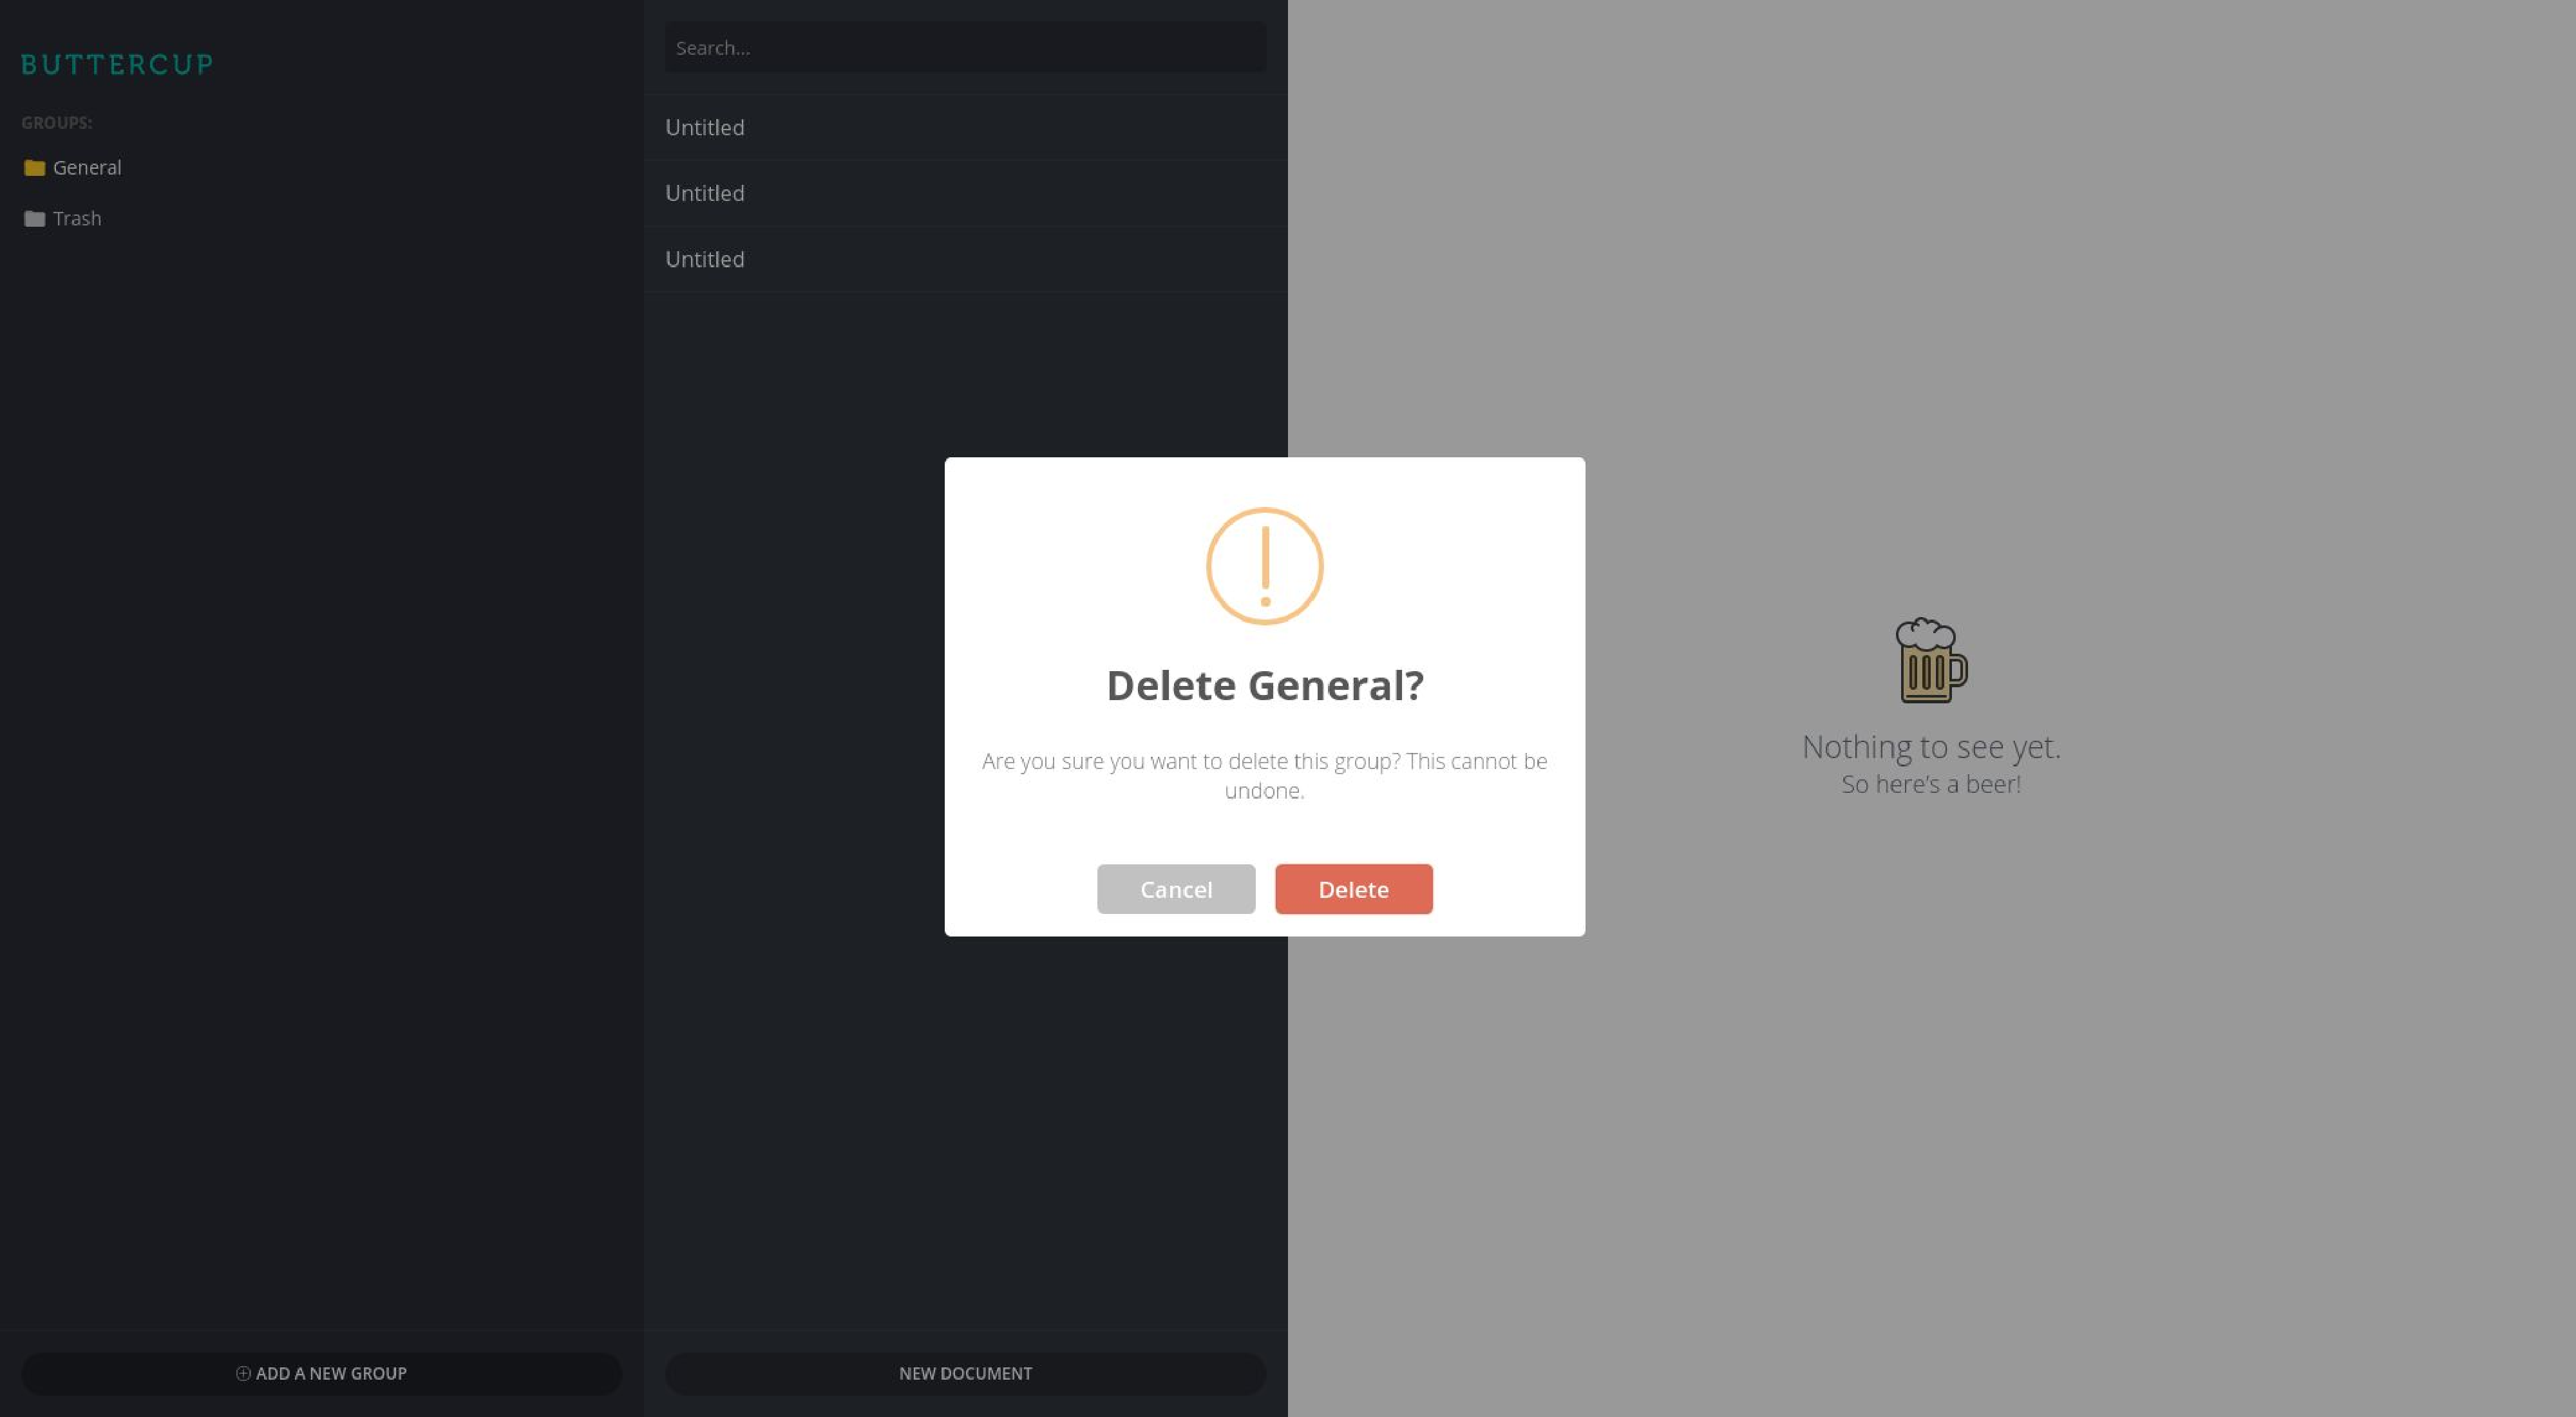
\includegraphics[scale=0.20]{8.pdf}
  \caption{ Экран удаление группы. }
  \label{fig:document:created_group:eith}
\end{figure}

\subsection{Управление записями в группе}
\label{sec:document:created_entry}

Добавление в записей производится при помощи панели активных действий в области записей, каждое из которых содержит свою валидационную модель. При попытке добавления некорректных данных пользователь получит предупреждение.

Также пользователь может отредактировать текущий список полей уже сделанной записи, добавив новые или удалив не актуальные. При попытке сохранить или обновить некорректные данные, будет показано сообщение об ошибке. Процесс работы с записью Untitled группы General представлен на рисунке~\ref{fig:document:created_entry:six}:
\begin{figure}[ht]
\centering
  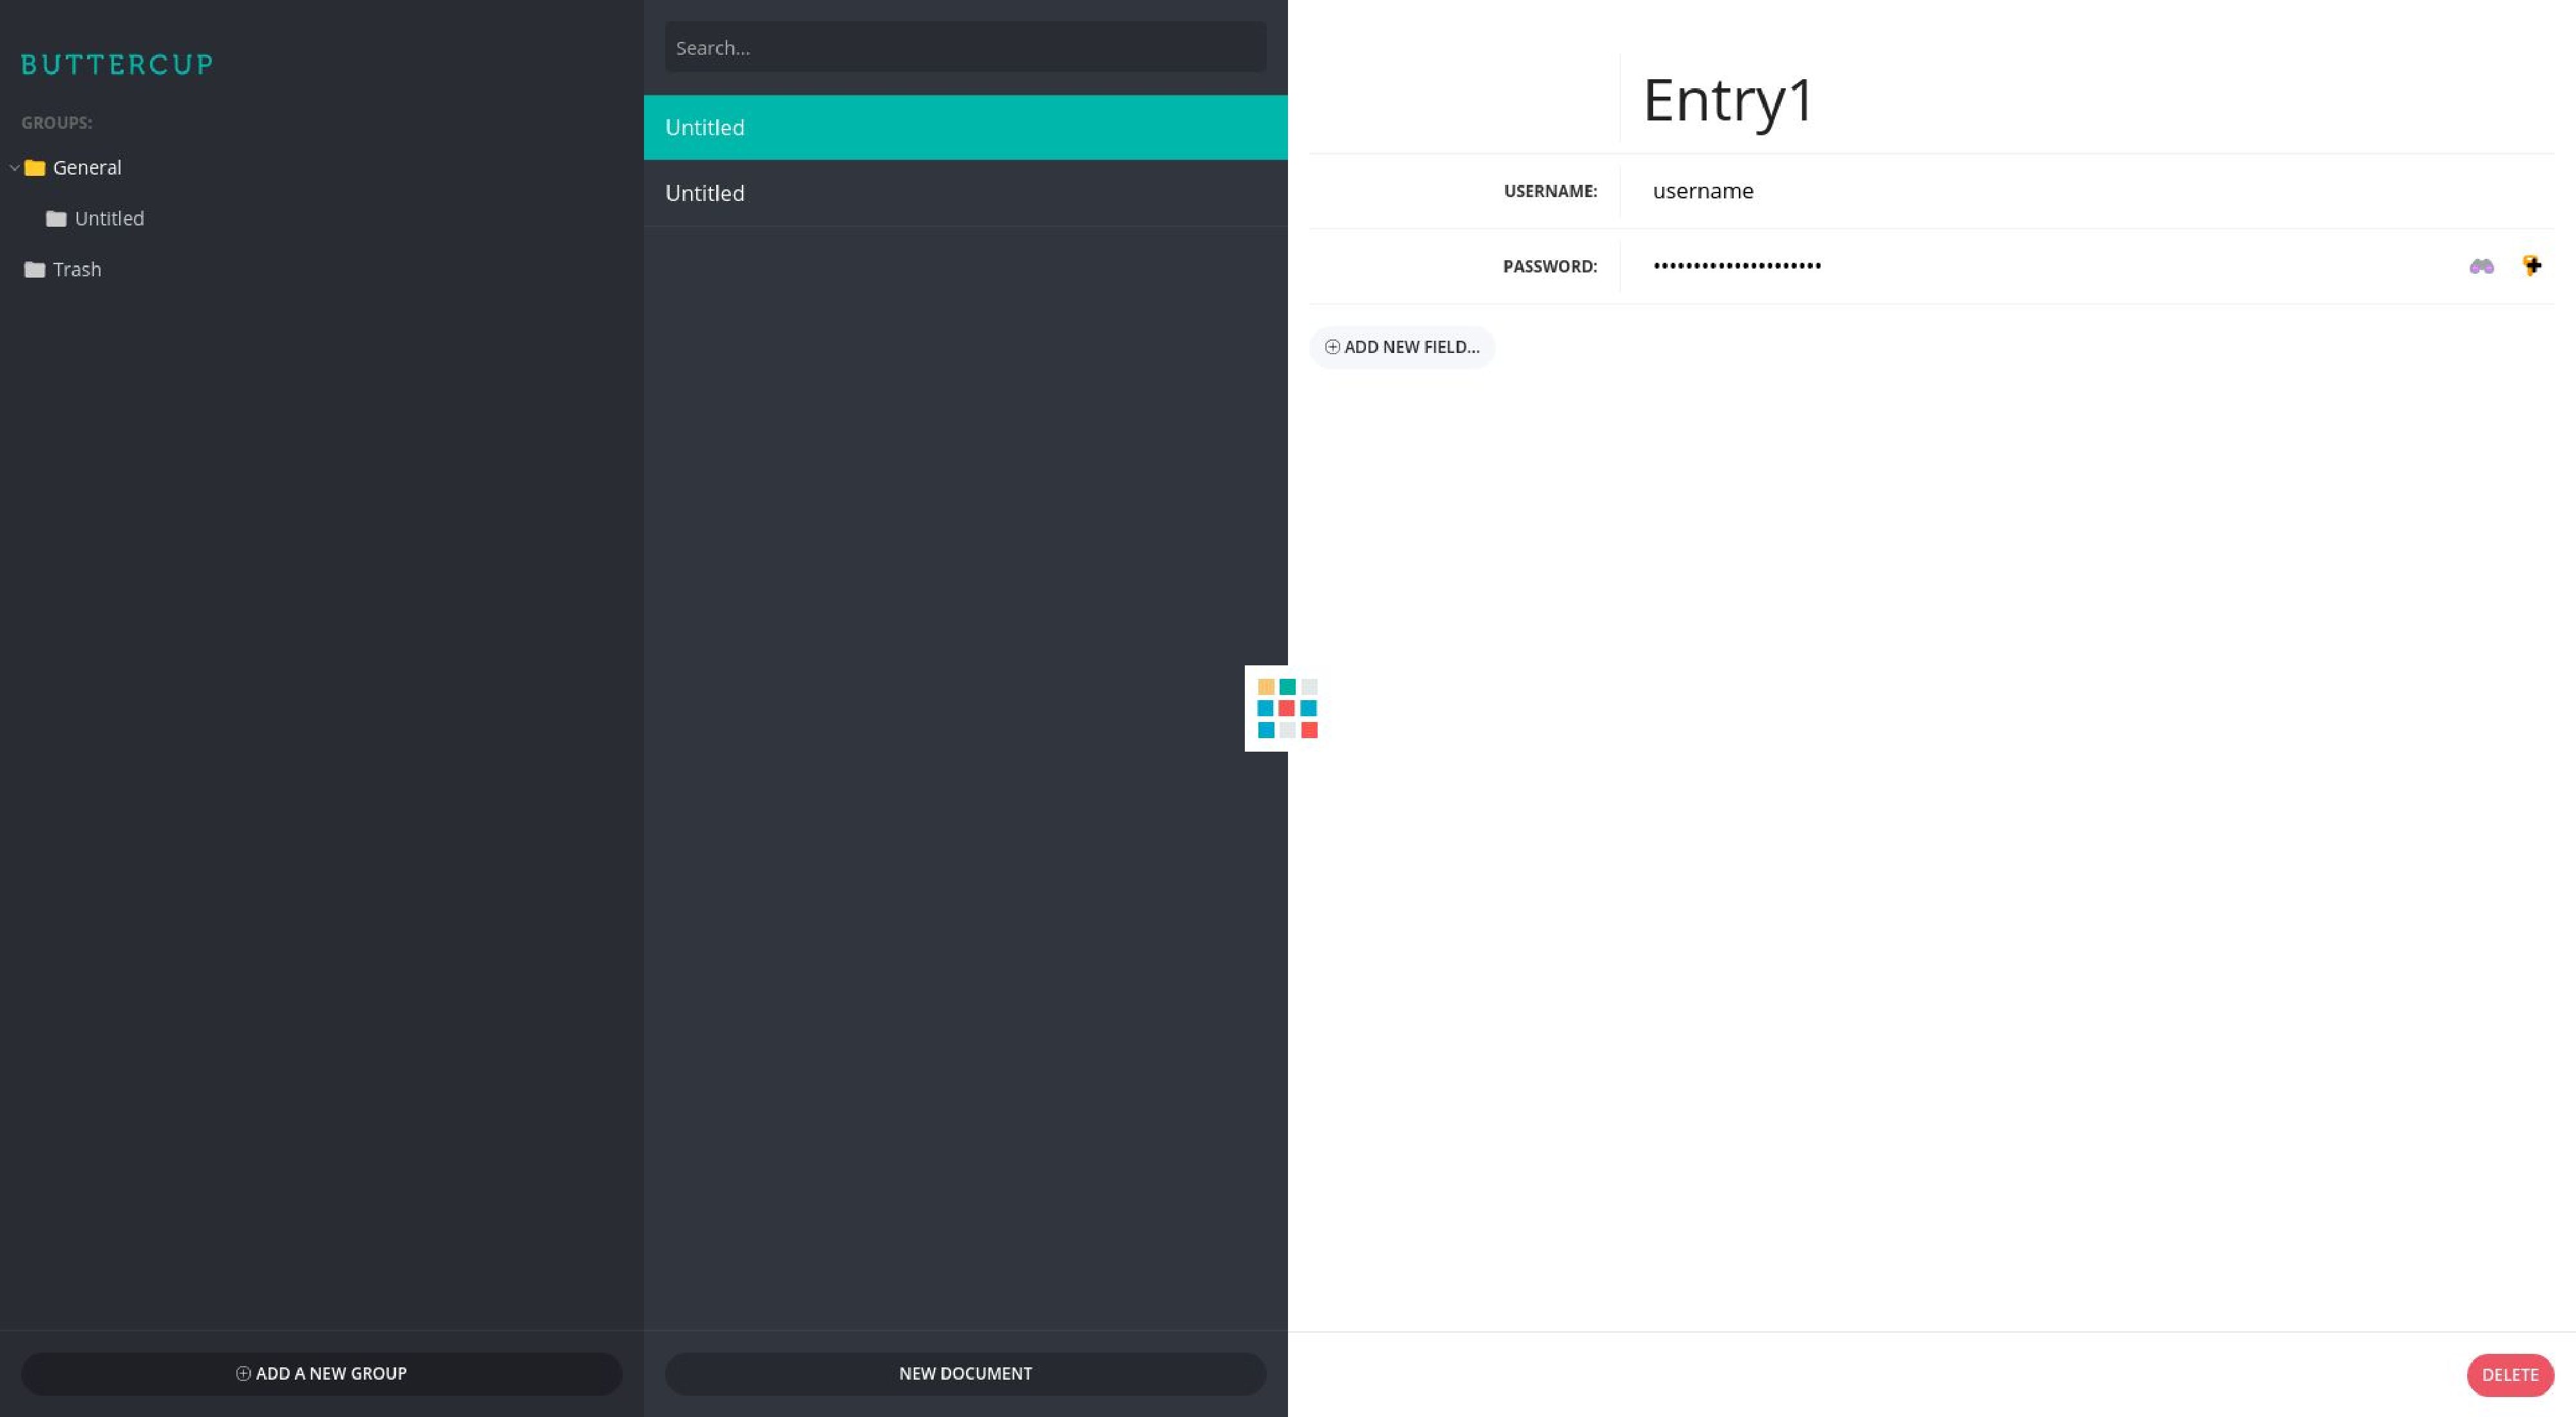
\includegraphics[scale=0.20]{6.pdf}
  \caption{ Экран работы c записью активной группы. }
  \label{fig:document:created_entry:six}
\end{figure}

Удаление записи в группе производится посредством ее собственной панели управления, состоящей из кнопок, предназначенных для удаления и смены ее имени, соотвественно. Процесс удаления записи Untitled группы General, представлен на рисунке~\ref{fig:document:created_entry:seven}.
\begin{figure}[ht]
\centering
  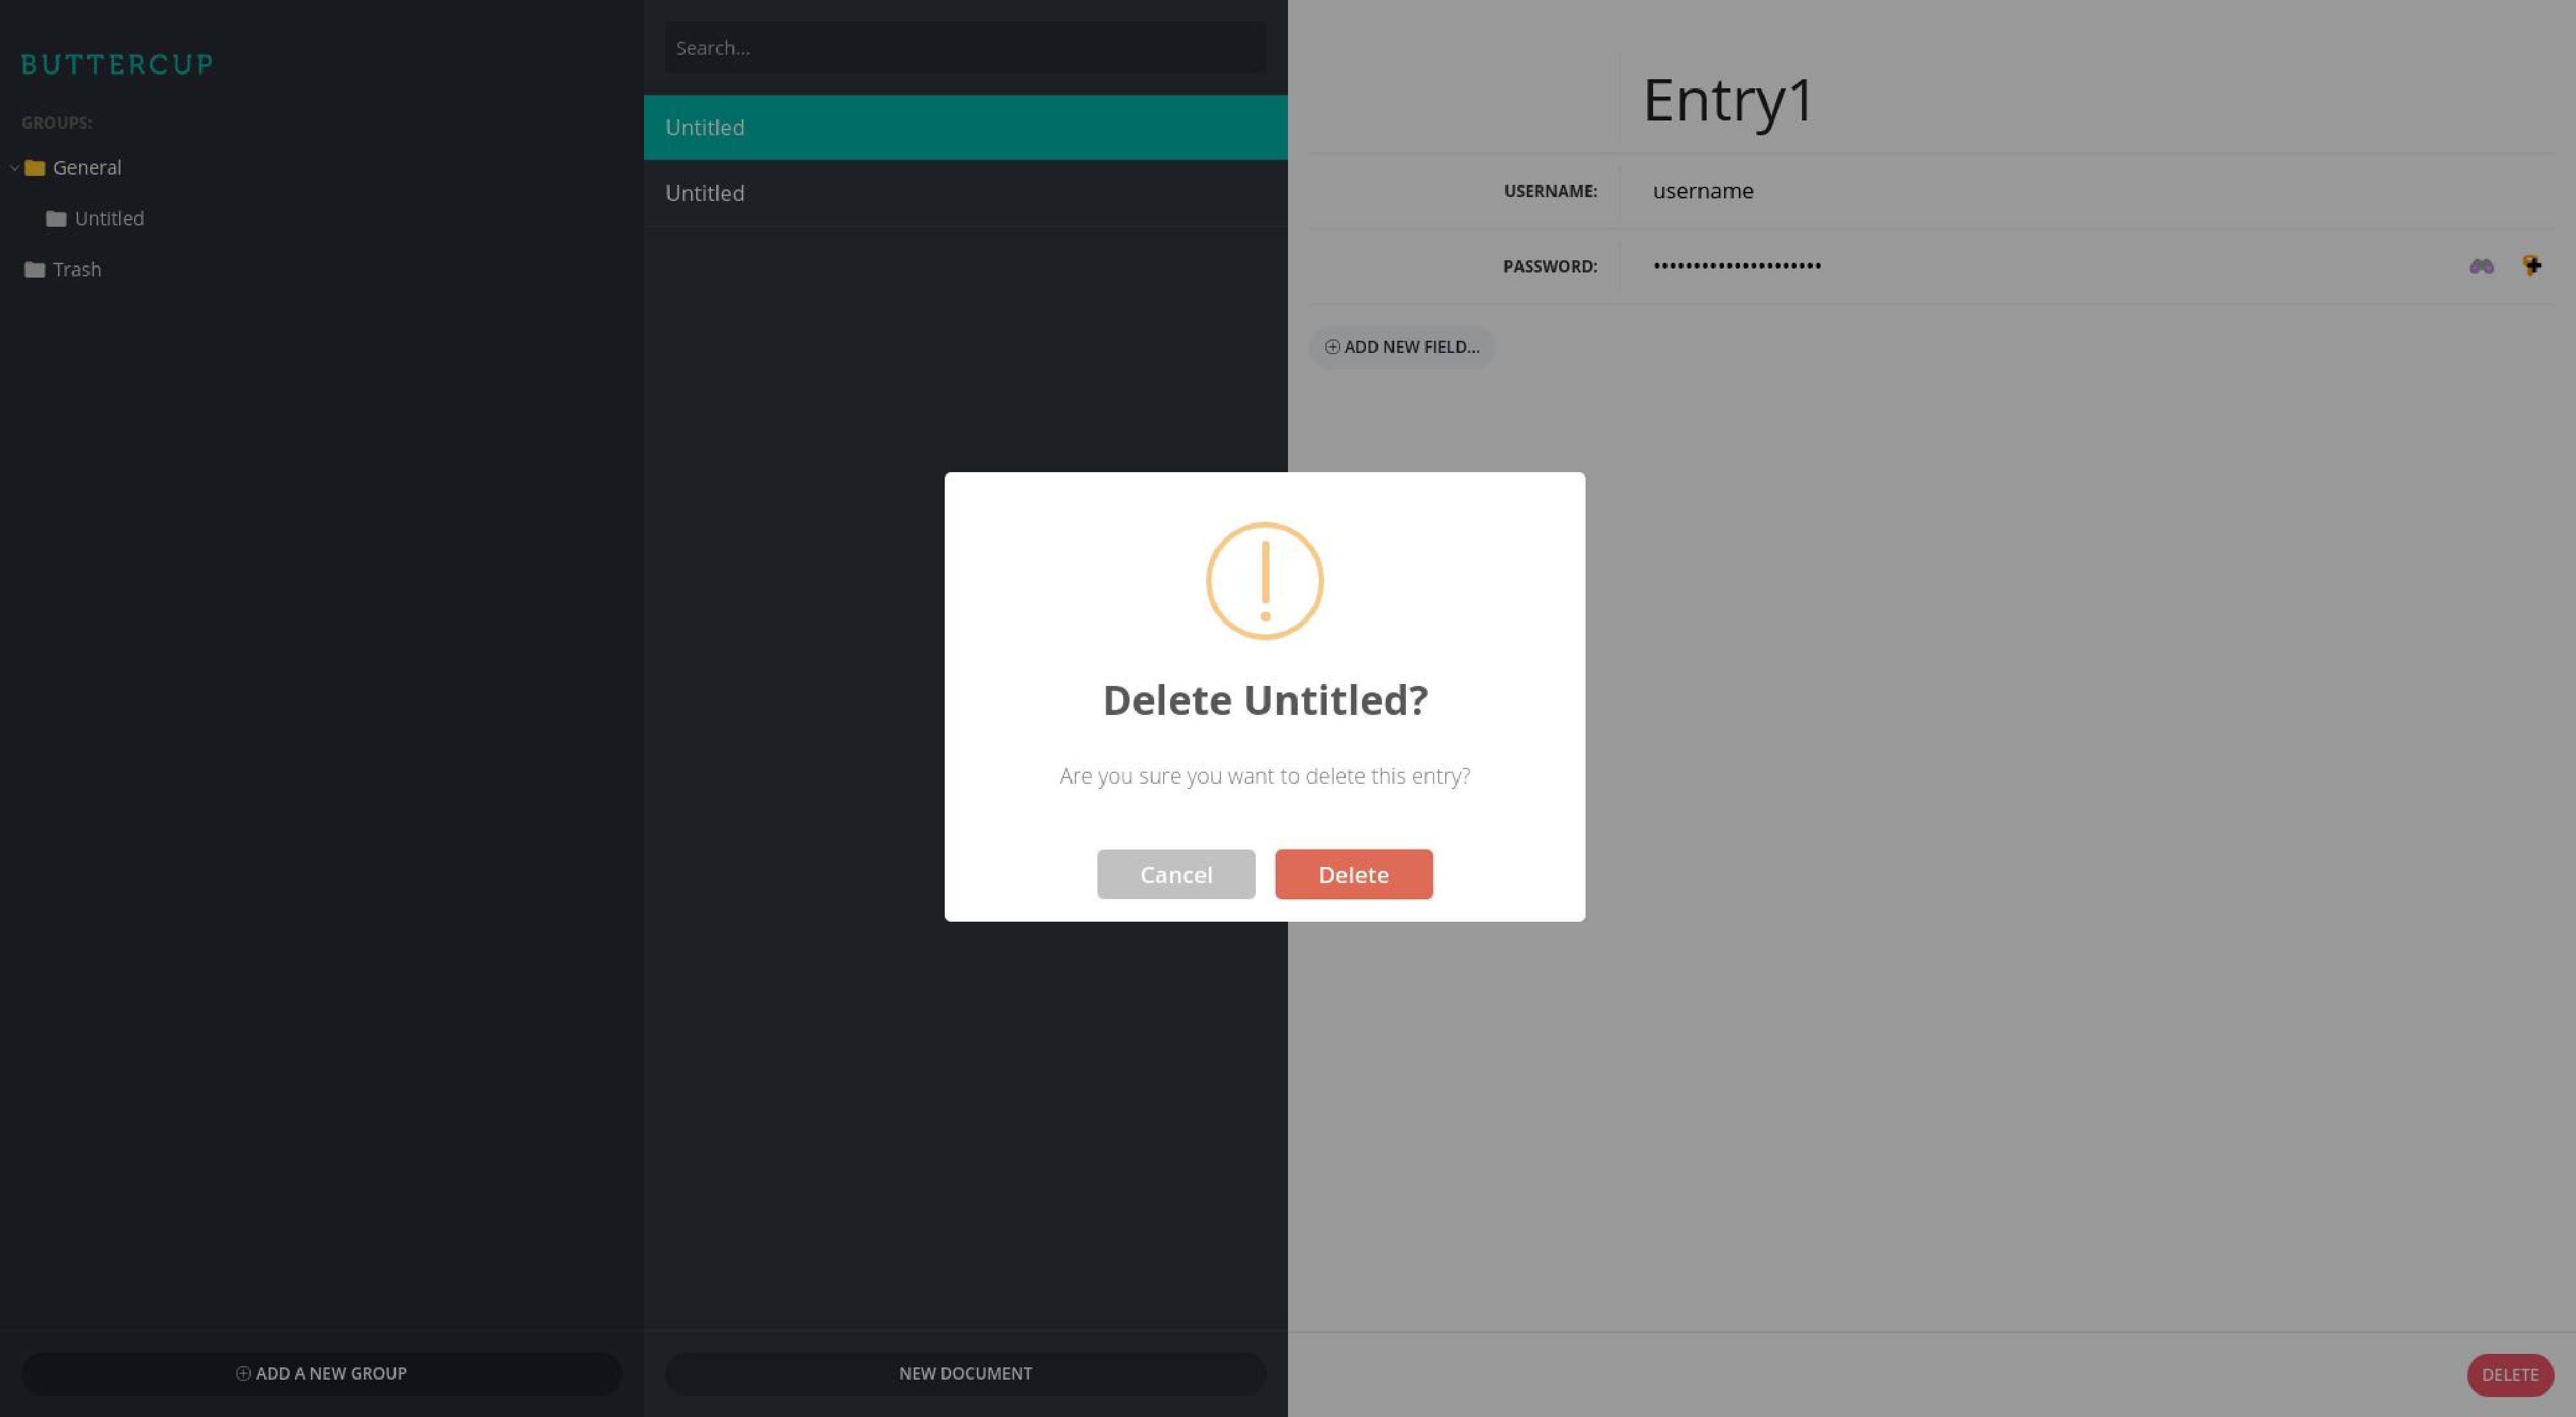
\includegraphics[scale=0.20]{7.pdf}
  \caption{ Экран удаление записи активной группы. }
  \label{fig:document:created_entry:seven}
\end{figure}

\newpage

Поле ввода пароля в области, предназначенной для работы с записью, содержит две иконочные кнопки: первая представляет пароль в читаемом для человека виде, вторая осуществляет генерацию случайного набора символов. В том случае, если была предпринята попытка генерации новой случайной последовательности в качестве пароля, пользователь получит диалоговое окно с предупреждением о вероятности замены текущего пароля, в случае его существования. Экран генерации нового пароля изображен на рисунке~\ref{fig:document:created_entry:ten}.

\begin{figure}[ht]
\centering
  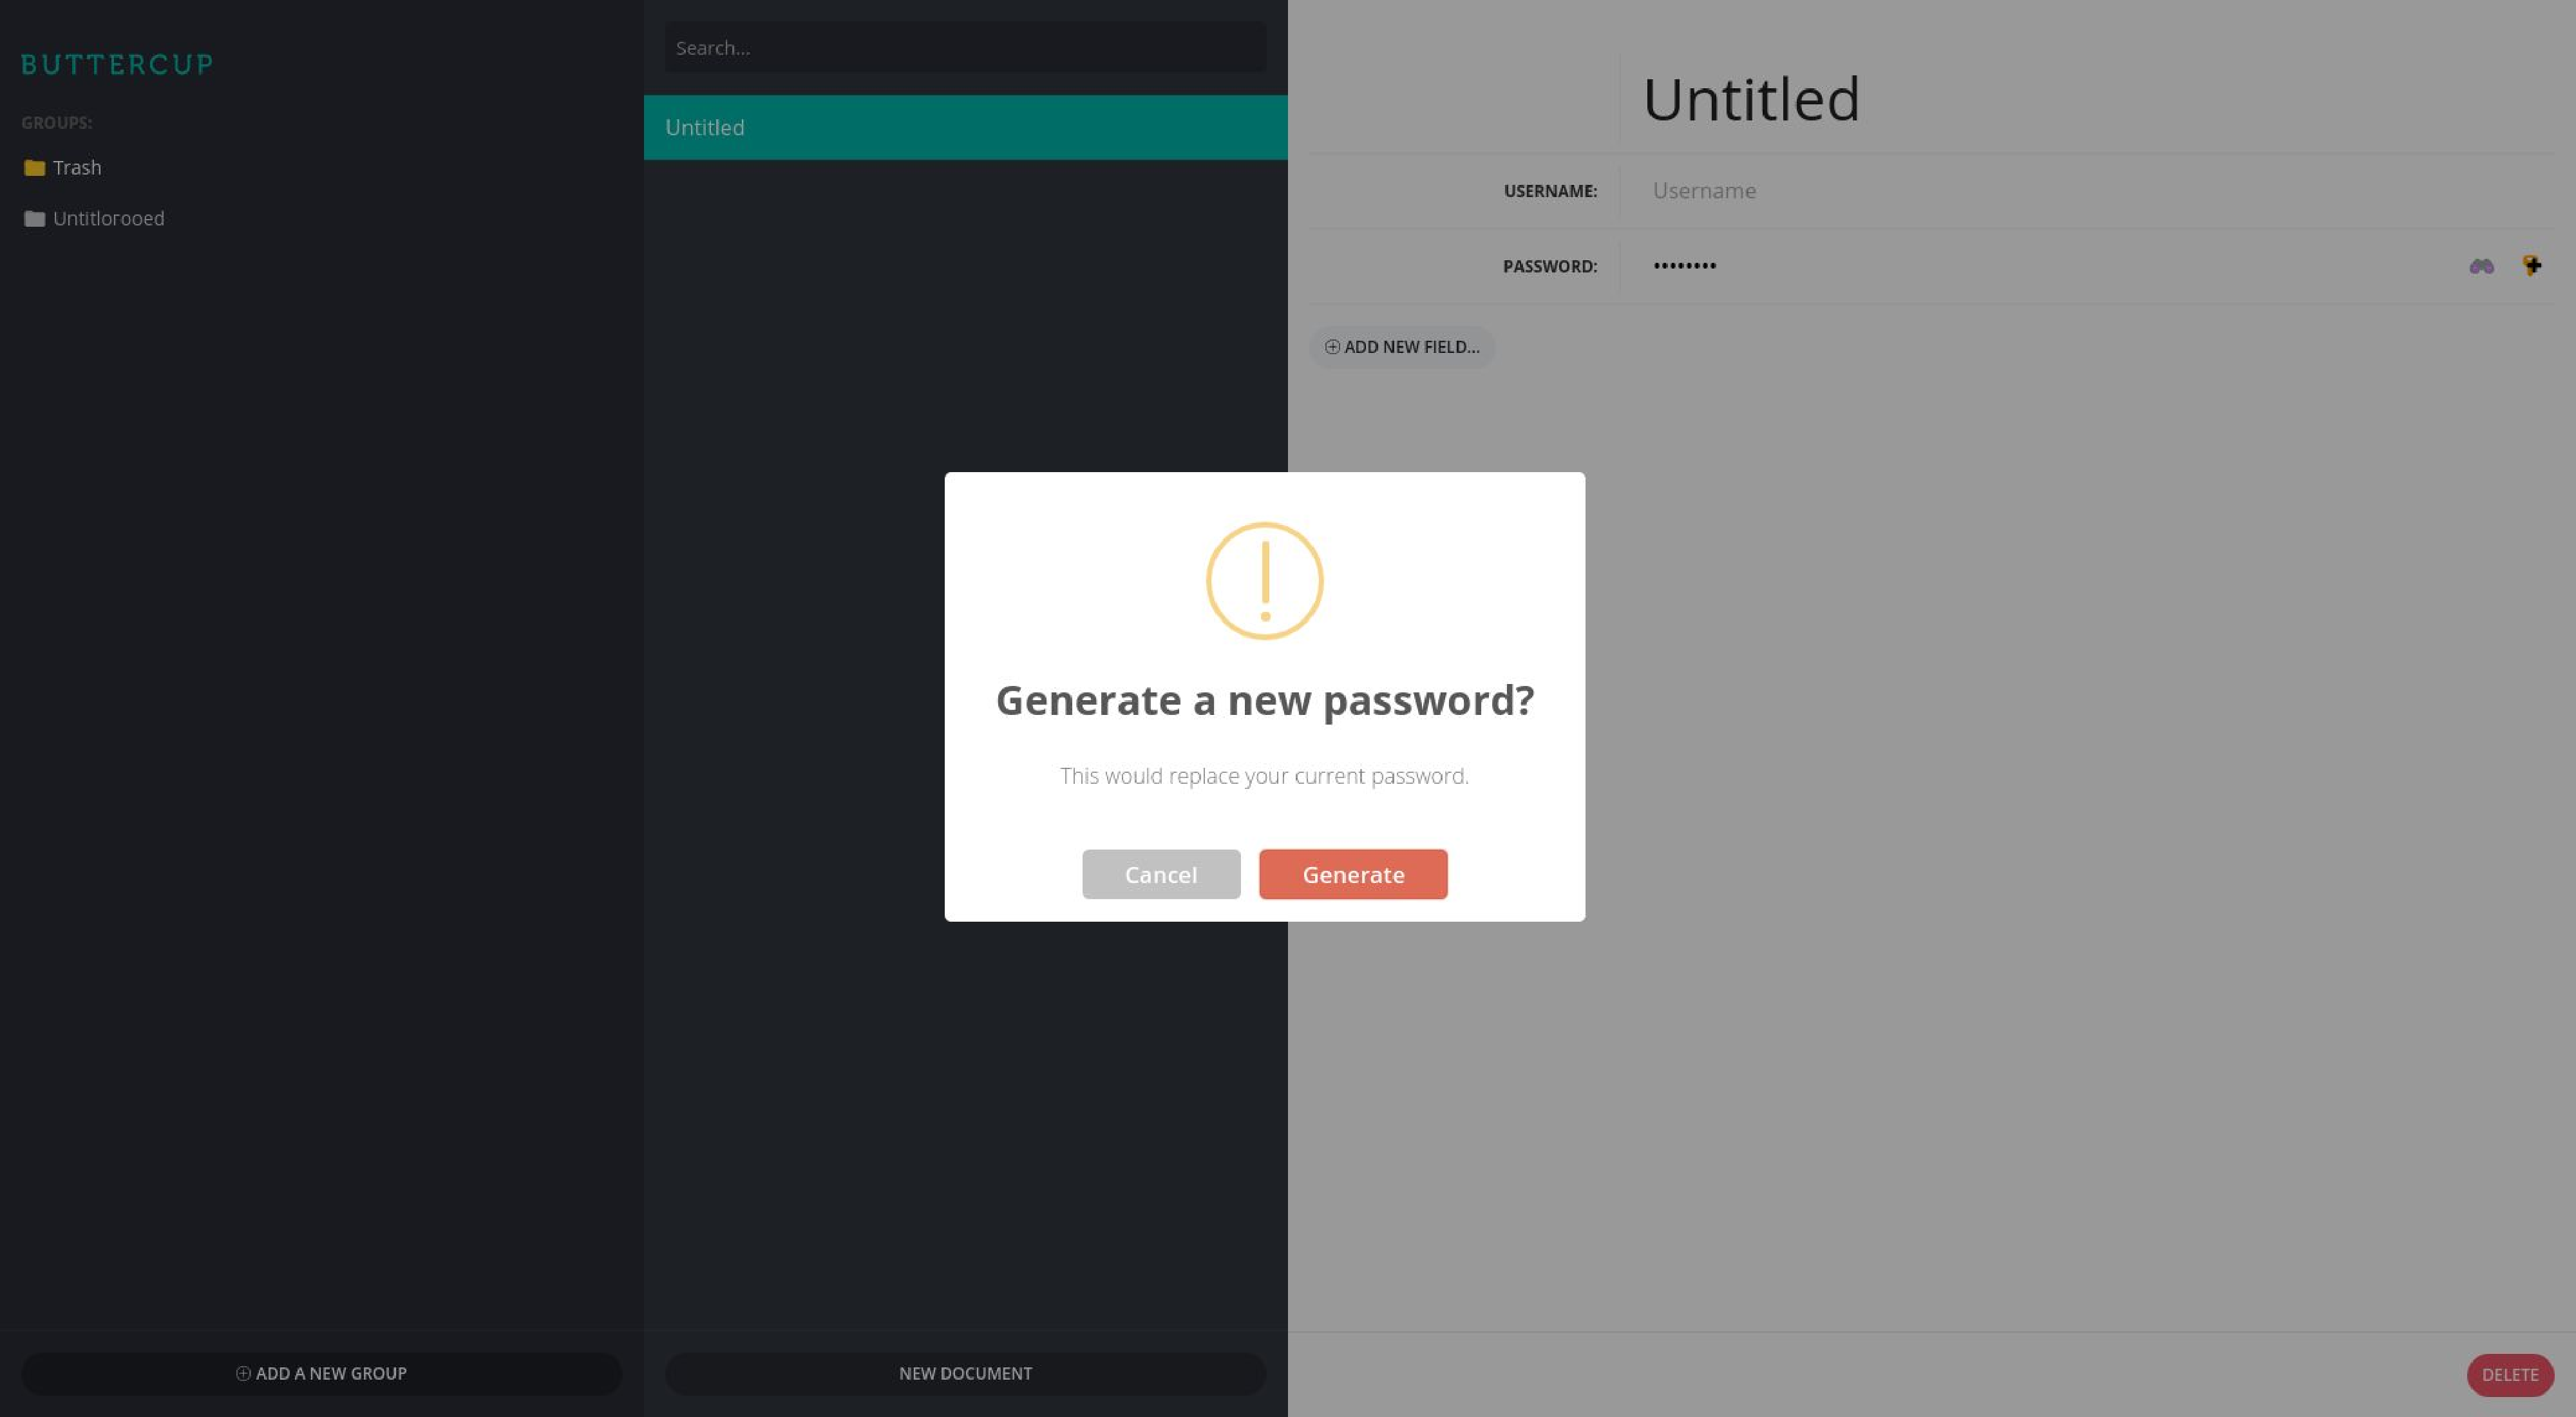
\includegraphics[scale=0.20]{10.pdf}
  \caption{ Экран генерации нового пароля. }
  \label{fig:document:created_entry:ten}
\end{figure}